\documentclass[a4paper,fleqn]{cas-dc}

\usepackage[UTF8,fontset=fandol]{ctex}
\usepackage[numbers,sort&compress]{natbib}
\usepackage{amsmath,amssymb}
\usepackage{unicode-math}
\setmathfont{STIX Two Math}
\usepackage{booktabs}
\usepackage{graphicx}
\usepackage{multirow}
\usepackage{threeparttable}
\usepackage{tabularx}
\usepackage{siunitx}
\usepackage{xcolor}
\usepackage{url}

\newcommand{\Thv}{\mathrm{Thv}}
\newcommand{\vect}[1]{\boldsymbol{#1}}
\newcommand{\todo}[1]{\textcolor{red!70!black}{【待补：#1】}}
\sisetup{detect-all,round-mode=places,round-precision=3}

\begin{document}
\let\WriteBookmarks\relax
\def\floatpagepagefraction{1}
\def\textpagefraction{.001}

\shorttitle{模组常规降温过程的历史--拓扑并行温度预测}
\shortauthors{作者姓名待补充}

\title[mode=title]{面向模组常规降温过程的历史--拓扑并行多步温度预测方法}

\author[1]{作者姓名待补充}
\cormark[1]
\affiliation[1]{organization={单位名称待补充},
  addressline={地址待补充},
  city={城市待补充},
  postcode={邮编待补充},
  country={中国}}
\cortext[1]{通讯作者}

\begin{abstract}
模组常规降温过程具有响应迟滞、变量强耦合和阀门作用沿管路逐级传播等特点，仅依赖当前温度或将全部测点压平输入单一时序网络，难以同时描述长期降温趋势、已知未来控制动作与工艺拓扑。本文构建一种面向未来第15个采样点的历史--拓扑并行温度预测框架。模型以过去60个采样点的温度、压力、流量和阀门开度编码系统历史状态，以当前工况下的固定有向管路图表示上游阀门到模组的传播路径，并独立编码从当前时刻起的15步已知阀门指令；三类表征在预测头中融合，输出模组平均温度相对于当前值的变化量，再恢复为绝对温度。为降低平稳区样本占优造成的零变化偏置，训练采用由训练集定义的快速降温加权Huber损失。独立批次实验表明，在10个随机种子下，历史窗口为60时获得最低完整测试集均方根误差（RMSE）1.180 K；继续增大窗口至65--120点未带来稳定收益。架构比较中，并行GRU--MLP--GNN的完整测试RMSE最低，为$1.142\pm0.049$ K；并行GRU--单调KAN--GNN为$1.150\pm0.044$ K，二者均优于GRU基线的$1.176\pm0.033$ K，而串行图--时序结构显著退化。考虑精度差异较小以及阀门边函数的可解释性，本文以并行GRU--单调KAN--GNN作为物理特征消融载体。20个因果构造特征使测试RMSE由$1.181\pm0.050$ K降至$0.960\pm0.033$ K，其中目标历史动态的独立贡献最稳定。结果说明，将时间记忆、已知未来控制和工艺拓扑分支建模，比在时序编码前强制压缩全部测点更适合该类缓变、分级控制的工业过程。本文当前结论限于开环离线预测；反事实单调性与跨工况外推将在后续实验中单独评估。
\end{abstract}

\begin{highlights}
\item 将历史动态、固定工艺拓扑与15步已知未来阀门序列并行编码。
\item 以10个随机种子的完整独立测试序列确定60点历史窗口。
\item 并行图--时序结构优于串行结构，物理特征使测试RMSE降低18.75\%。
\end{highlights}

\begin{keywords}
模组常规降温 \sep 多步温度预测 \sep 门控循环单元 \sep 图神经网络 \sep Kolmogorov--Arnold网络 \sep 物理引导机器学习
\end{keywords}

\maketitle

\section{引言}\label{sec:introduction}

模组常规降温是一个典型的慢动态工业过程。多个冷源经阀门调节、汇流和管路传输后进入模组，温度响应同时受历史热状态、阀门动作、流量与压力变化以及沿程换热影响。严格的热力学或流程仿真能够提供较强的物理一致性，但瞬态求解通常需要反复积分；当预测模型需要在较短时间内评估多组候选控制序列时，计算代价可能成为限制。神经代理模型能够将复杂动态映射压缩为快速前向推理，因此已被广泛用于工业软测量、温度预测和控制辅助\citep{faridi2023spatiotemporal,tan2022multistep,costa2024multistep}。

这一任务的困难不只是时间序列拟合。首先，降温记录包含较长的平稳或缓变区，若直接预测绝对温度，模型可以通过复制当前值获得较低的整体误差，却不能保证捕捉控制动作后的温度变化。其次，阀门具有明确的分级拓扑：上游阀门改变可用冷量和流通能力，下游阀门进一步决定进入模组的作用强度。将所有变量作为无结构向量输入循环网络，会弱化这种传播关系。再次，实际训练数据只覆盖有限操作轨迹；纯数据驱动模型即使在同分布数据上误差较低，也可能在控制干预下给出方向错误的响应。已有研究分别从多步循环预测、空间特征分解、图消息传递和单调物理约束等角度处理上述问题，但很少在同一工业温度预测框架中同时区分历史状态、固定工艺拓扑和已知未来控制。

本文研究目标是建立一个可进一步嵌入模型预测控制的快速温度预测模型，但本阶段仅讨论传统开环时序预测性能，不讨论闭环控制效果。本文贡献概括如下：
\begin{enumerate}
  \item 构造因果对齐的残差预测任务：使用截至当前时刻的历史测量和从当前时刻起的15步阀门指令，预测未来第15个采样点的模组平均温度变化量；未来非控制测量不进入输入。
  \item 提出历史--拓扑并行模型：GRU提取长时间趋势，固定有向GNN表达管路传播，单调样条KAN仅作用于阀门边门控，未来控制序列由独立分支编码，避免物理拓扑表征提前替代全部历史信息。
  \item 采用跨文件严格隔离的实验协议，以10个随机种子的完整独立测试序列确定历史窗口，并比较基线、并行和串行架构；进一步通过分组消融识别构造特征的有效部分。
\end{enumerate}

\section{相关研究进展}\label{sec:related}

\subsection{机理模型与数据驱动代理}

机理模型通过质量、动量和能量守恒描述过程动态，优点是变量含义清晰且便于检查约束；不足是复杂设备、未知边界条件和沿程漏热会显著增加建模与标定成本。对于空间场演化，Fourier神经算子等代理模型可在仿真数据上学习算子映射，并在多相流案例中获得比CFD快3--4个数量级的推理速度\citep{guida2026fno}。然而，神经算子通常依赖规则空间场或大规模仿真样本，而本文数据由稀疏管路测点构成，拓扑先验比规则网格先验更直接。

\subsection{循环网络与多步温度预测}

LSTM通过门控记忆缓解长时依赖中的梯度衰减\citep{hochreiter1997lstm}，GRU则以更紧凑的门控结构实现相似的状态更新\citep{cho2014gru}。在流化床温度预测中，动态LSTM被用于同时预测不同位置和不同提前量的温度，预测时距增加时误差随之增大；GRU在部分工况下收敛更快，但并不存在对LSTM的普遍优势\citep{faridi2023spatiotemporal}。在再热蒸汽温度预测中，研究者对回看步数、网络层数和隐藏节点数逐项寻优，并一次输出未来5步温度\citep{tan2022multistep}。针对控制与优化用途，直接多步模型还能减少单步递归反馈造成的误差传播和预测不确定性\citep{costa2024multistep}。

这些工作证明了循环网络对慢动态温度过程的适用性，但多数模型仍把测点作为平坦特征向量，且未显式区分“历史测量”与“决策时已知的未来控制”。本文保留GRU作为历史趋势编码器，同时将未来阀门轨迹作为独立条件输入。

\subsection{空间耦合、图表示与特征选择}

工业软测量研究已开始将输入空间划分或分布式特征提取与LSTM结合，以同时处理非线性、动态性和空间耦合\citep{he2025nisrdelm}。图神经网络通过沿边聚合相邻节点信息，为结构化关系提供统一的消息传递形式\citep{gilmer2017mpnn}。对于具有明确流向的管路系统，固定有向图还能避免从有限数据中重新学习本已知的连接关系。

另一方面，更多特征并不必然提高跨工况性能。TempCaFe将时间因果发现与领域知识结合，在数据中心多个预测任务中用不到原特征三分之一的变量获得更好的干预后鲁棒性\citep{zapata2026tempcafe}。这提示特征价值不能只由单次随机划分的整体RMSE判断，而应在独立工况和成组消融中验证。

\subsection{物理约束、单调网络与连续时间模型}

物理引导学习可通过方程残差、结构约束或软惩罚将先验嵌入网络\citep{raissi2019pinn}。单调约束尤其适合描述“在其他条件固定时，控制量增大不应引起相反方向响应”的局部规律。受约束单调网络可通过权重符号和专门激活函数保证函数类的单调性\citep{runje2023monotonic}；针对冷水机的MonoPINN则表明，单调物理损失可能轻微牺牲插值精度，却能改善跨工况外推\citep{tang2026monopinn}。

KAN将可学习的一元函数放置在连接边上，为低维非线性关系提供可视化接口\citep{liu2025kan}。因此本文不把KAN作为替代全部时序网络的通用模块，而只用它表示“阀门开度--边导通强度”的一元关系，并通过正增量参数化保证该边函数非减。Neural ODE能够连续描述隐状态演化\citep{chen2018neuralode}，近期也有工作协调离散历史编码与连续动力学以提升分布偏移下的适应性\citep{li2026npc}。但本文数据等间隔采样，当前核心问题是分级拓扑与有限工况，而非不规则采样，因此暂不引入ODE求解器，以避免增加尚不能由实验单独归因的复杂度。

表\ref{tab:literature}总结了主要路线及其与本文的关系。

\begin{table*}[t]
\centering
\caption{相关建模路线的能力、局限及本文处理方式。}
\label{tab:literature}
\begin{tabularx}{\textwidth}{@{}p{2.6cm}p{3.4cm}p{4.0cm}X@{}}
\toprule
路线 & 主要优势 & 主要局限 & 本文中的处理 \\
\midrule
机理/瞬态仿真 & 物理含义明确，可检查守恒与边界 & 建模、标定和多方案求解成本高 & 仅提取管路连接、流向和热力学代理，不直接替代瞬态求解 \\
LSTM/GRU多步预测 & 擅长表示历史迟滞，可直接预测未来状态 & 平坦输入弱化测点拓扑；易受平稳样本主导 & GRU仅负责编码历史趋势，并预测温度变化量 \\
空间特征分解或因果选择 & 降低冗余，提高跨工况鲁棒性 & 依赖划分或因果发现稳定性，未必表示真实传播路径 & 用领域知识固定有向图，并以独立批次做特征组消融 \\
GNN & 显式利用节点和边关系 & 串行使用可能过早压缩原始历史信息 & 比较串行与并行结构，保留GRU直达预测头 \\
单调约束/KAN & 提高局部物理一致性和可解释性 & 错误或全局化的单调假设会限制拟合 & 仅约束阀门自身边函数，其他上下文由无约束网络拟合 \\
Neural ODE/FNO & 适合连续时间或规则空间场代理 & 求解器或场数据要求提高复杂度 & 作为后续扩展，不纳入当前等间隔稀疏测点主模型 \\
\bottomrule
\end{tabularx}
\end{table*}

\section{问题定义与数据协议}\label{sec:data}

\subsection{过程变量与预测目标}

系统由两条G支路和一条A支路提供不同温度水平的工质。G支路的上游控制阀为CV8300和CV8313，汇合后由CV8310控制进入主混气管路；CV8311和CV8312连接到其他支路。A支路由CV8351控制。主混气管路依次布置TE8351、TE8352和TE8353等测点，随后通过EC-V2和COOLDOWN两个模组侧阀门进入模组。本文以模组多个测点的平均温度$\Thv$为预测目标，TE8353视为模组入口附近的上游温度信息。

原始历史变量共20个，包括5个温度相关过程量（TE8310、TE8351、TE8352、TE8353和$\Thv$）、3个压力变量、1个流量变量、8个阀门开度以及Tef、Tcd和DTbr等模组状态量。压力、流量和温度的单位分别为bar、g/s和K；阀门开度使用百分数记录。负的阀门漂移值在预处理阶段截断为0，但合法的0\%开度保留。

采样周期为$\Delta t=10$ s。给定历史窗口长度$L$和预测步长$H=15$，历史输入为
\begin{equation}
\vect X_t=[\vect x_{t-L+1},\ldots,\vect x_t],
\end{equation}
已知未来控制为
\begin{equation}
\vect U_t=[\vect u_t,\vect u_{t+1},\ldots,\vect u_{t+H-1}],
\end{equation}
其中$\vect u$仅包含8个阀门开度。模型不读取$t$之后的温度、压力或流量。监督目标采用温度变化量
\begin{equation}
\begin{aligned}
\Delta \Thv_{t,H}&=\Thv_{t+H}-\Thv_t,\\
\widehat{\Thv}_{t+H}&=\Thv_t+\widehat{\Delta \Thv}_{t,H}.
\end{aligned}
\label{eq:delta}
\end{equation}
这一设计把持久性预测明确化为$\widehat{\Delta \Thv}=0$，便于检查模型是否真正学习到未来变化。

\subsection{数据划分与防泄漏约束}

数据按完整运行批次划分，而不是随机打散时间点。训练使用0623-BACK、0715-ALL、251130、251226、260118和260403六个父数据源，0617因缺少模组侧阀门而在训练脚本中排除；验证集为Original 260501；测试集为Original 0715-BACK的完整可预测序列。0715-BACK包含降温后的复温及再次降温过程，阀门变化和状态反转较多，因此被用作跨运行轨迹的独立测试，而不是普通平稳降温样本。

过滤在扩增之前完成。训练父数据保留原始版本及两个轻量扩增版本；验证和测试只使用原始版本。所有滑动窗口必须位于同一文件和同一连续有效片段内，不跨文件、不跨过滤断点。标准化器、快速降温阈值和目标尺度仅由排除0617后的训练数据拟合。模型选择只使用260501验证集，待所有架构和随机种子完成且结果冻结后，才统一读取0715-BACK测试集。架构比较使用306,543个训练窗口、25,600个验证窗口和10,659个完整测试窗口。

\begin{table}[t]
\centering
\caption{数据划分与用途。}
\label{tab:split}
\begin{tabular}{@{}p{1.45cm}p{4.1cm}p{1.8cm}@{}}
\toprule
划分 & 父数据源 & 用途 \\
\midrule
训练 & 0623-BACK、0715-ALL、251130、251226、260118、260403 & 参数与标准化拟合 \\
验证 & Original 260501 & 早停与模型选择 \\
测试 & Original 0715-BACK & 冻结后的最终评价 \\
\bottomrule
\end{tabular}
\end{table}

\section{历史--拓扑并行预测方法}\label{sec:method}

\subsection{总体结构}

模型由历史编码分支、物理图分支和未来控制分支组成。三条分支分别回答三个问题：系统此前如何变化、当前测点沿已知管路如何连接、接下来15步将施加什么阀门动作。与串行“逐时刻图编码后再进入GRU”的方案不同，并行结构允许GRU直接访问完整原始历史，GNN只补充当前工况的拓扑摘要，从而降低拓扑编码误差在时间轴上重复累积的风险。三条分支的隐表示拼接后，经融合网络输出式\eqref{eq:delta}中的温度变化量。
% 最终模型冻结后，在此处补充整体架构图；当前初稿不使用临时示意图。

\subsection{历史动态编码}

历史分支采用单层GRU，隐藏维度为64。对标准化后的历史序列$\vect X_t$递推得到状态$\vect h_t^{\mathrm{gru}}$。GRU相较LSTM参数更少，且在本文10种子比较中，GRU基线和GRU并行模型的平均测试误差均略低于相应LSTM版本，因此后续主模型保留GRU。

\subsection{固定有向工艺图}

物理图包含11个节点：G1源、G2源、G汇流、G主路、两条分支、A源、混气后测点、主干中间测点、模组入口和模组平均温度。图中11条有向边按实际流向连接，上游控制阀被放置在对应边上。节点特征由当前温度、压力、流量、局部阀门和可用性掩码组成；边特征包含当前开度、一步开度变化、温压流上下文及相关并列阀门状态。

对边$i\rightarrow j$，一次拓扑消息传递可写为
\begin{equation}
\begin{aligned}
\vect m_{i\rightarrow j}
  &=g_{ij}(a_{ij},\vect c_t)\vect W_m\vect z_i,\\
\vect z'_j
  &=\mathrm{LN}\!\left[\vect z_j+
    \phi\!\left(\vect z_j,\sum_i\vect m_{i\rightarrow j}\right)\right],
\end{aligned}
\label{eq:message}
\end{equation}
其中$a_{ij}$为阀门开度，$\vect c_t$为温度、压力、流量和相关阀门上下文，$g_{ij}\geq0$为边门控，$\phi$为两层感知机。消息按管路拓扑顺序传播两遍，最终汇集模组、混气后、入口和全图平均状态，形成64维图表征$\vect h_t^{\mathrm{graph}}$。

\subsection{MLP与单调KAN边门控}

MLP边门控直接由边属性学习非负导通强度，表达能力强，但不能保证阀门自身开度增大时边门控不减。单调KAN版本将阀门自身作用与其他上下文分开：
\begin{equation}
g_{ij}(a_{ij},\vect c_t)=s_{ij}(a_{ij})\,\mathrm{softplus}\bigl(q_{ij}(\vect c_t)\bigr),
\end{equation}
其中$q_{ij}$为无约束上下文网络，$s_{ij}$是在$[0,1]$开度区间定义的一维分段线性样条。各相邻节点增量通过softplus参数化为正数，因此
\begin{equation}
\frac{\partial s_{ij}(a)}{\partial a}\geq0.
\end{equation}
该约束只表示“阀门开大不降低本边的导通能力”，并不直接约束最终温度对任一阀门全局单调，因为最终响应还取决于入口温度、压差、其他阀门和混合状态。由此避免把局部合理先验错误扩展为全局温度规律。

\subsection{已知未来控制与特征融合}

未来控制分支将$15\times8$的阀门序列展平后，经线性层、SiLU和dropout编码为32维状态$\vect h_t^u$。最终预测为
\begin{equation}
\widehat{\Delta\Thv}_{t,H}=psi\left(
[\vect h_t^{\mathrm{gru}};\vect h_t^{\mathrm{graph}};\vect h_t^u]
\right),
\end{equation}
其中$\psi$包含64维融合层和标量输出层。这里使用$\vect u_t$至$\vect u_{t+14}$，不使用与目标点同时发生的$\vect u_{t+15}$，与离散状态转移对齐。

\subsection{因果构造特征}

数据表预先生成20个推荐构造特征，训练时按组选择，全部只使用当前或历史信息。表\ref{tab:features}给出其物理来源。G支路代理量不是实测质量流量，300 K参考制冷量也不是制冷机额定功率，本文仅将它们作为可消融的低阶物理坐标。氦气焓由CoolProp计算\citep{bell2014coolprop}。

\begin{table*}[t]
\centering
\caption{构造特征组、代表性定义与物理目的。}
\label{tab:features}
\begin{tabularx}{\textwidth}{@{}p{3.0cm}p{6.8cm}X@{}}
\toprule
特征组（数量） & 代表性定义 & 作用 \\
\midrule
目标历史动态（4） & $T_t-T_{t-1}$；$(T_t-T_{t-59})/(590/60\ \mathrm{min})$，$T\in\{\mathrm{TE8353},\Thv\}$ & 显式给出局部增量和约10 min历史斜率 \\
G主路流通指令代理（2） & 两个串联阀等效开度$\times\sqrt{\max(P_{8310}-P_{8351},0)}$ & 表示G1/G2支路的相对导通与压差驱动，不冒充实测流量 \\
混气热驱动（4） & G1/G2流通代理$\times$混气温差；CV8351开度$\times(TE8351-4.6)$；CV8351一阶差分 & 表示不同名义入口温度与A支路动作对混气状态的影响 \\
混气后制冷桥接（2） & $h(300\mathrm{K},P_{8351})-h(T_{8351},P_{8351})$及其与$FT8351$的乘积 & 将TE8351处温压流联系为相对300 K参考的焓差和流量加权代理 \\
主干状态差（3） & $TE8351-TE8352$、$TE8352-TE8353$、$PT8351-PT8352$ & 表示沿程温差和压差 \\
模组耦合（3） & $\Thv-TE8353$、$FT8351(\Thv-TE8353)$、$\Thv-TE8310$ & 表示入口、流量驱动及状态机参考温差 \\
模组阀门动态（2） & $\Delta EC\mbox{-}V2$、$\Delta COOLDOWN$ & 标记末级控制动作 \\
\bottomrule
\end{tabularx}
\end{table*}

\subsection{训练目标}

由于平稳样本多于快速降温样本，采用训练集$\Delta\Thv$的第10百分位$q_{0.1}$定义快速降温样本。其权重设为3，其余样本权重为1：
\begin{equation}
\begin{aligned}
w_i&=1+2\,\mathbb I(\Delta\Thv_i\leq q_{0.1}),\\
\mathcal L&=\frac{\sum_i w_i\,\ell_{\mathrm{Huber}}(\hat y_i-y_i)}
                  {\sum_i w_i}.
\end{aligned}
\end{equation}
Huber损失兼顾小误差区的平滑优化和对残余异常点的稳健性\citep{huber1964robust}。优化器为Adam\citep{kingma2015adam}，初始学习率$10^{-3}$、权重衰减$10^{-5}$、批大小256、最大100轮，早停耐心值为12。历史、控制和目标分别标准化，所有统计量只由训练集拟合。

\section{实验结果}\label{sec:results}

\subsection{评价方式}

所有主结果均在0715-BACK完整测试序列的10,659个窗口上计算。报告RMSE、平均绝对误差（MAE）、绝对误差95百分位（P95）、最大绝对误差、偏差和$R^2$。模型以10个随机种子重复训练，表中给出均值$\pm$样本标准差。持久性基线直接令$\widehat{\Thv}_{t+15}=\Thv_t$，其测试RMSE为1.978 K。

\subsection{历史窗口长度选择}

为保证不同历史窗口比较同一批预测起点，所有窗口共享按最大回看范围确定的候选终点。测试的$L$为15、30、40、45、50、55、60、65、70、75、90和120。图\ref{fig:lookback}显示，RMSE从$L=15$的$1.256\pm0.038$ K总体下降；$L=60$时达到最低均值$1.180\pm0.039$ K。继续增加至65、90和120时，均值分别为1.185、1.188和1.192 K，没有形成稳定改善，方差也未持续缩小。因此选择$L=60$：它覆盖600 s历史，达到观测范围内的数值最低点，同时避免更长序列带来的训练成本。

\begin{figure*}[t]
  \centering
  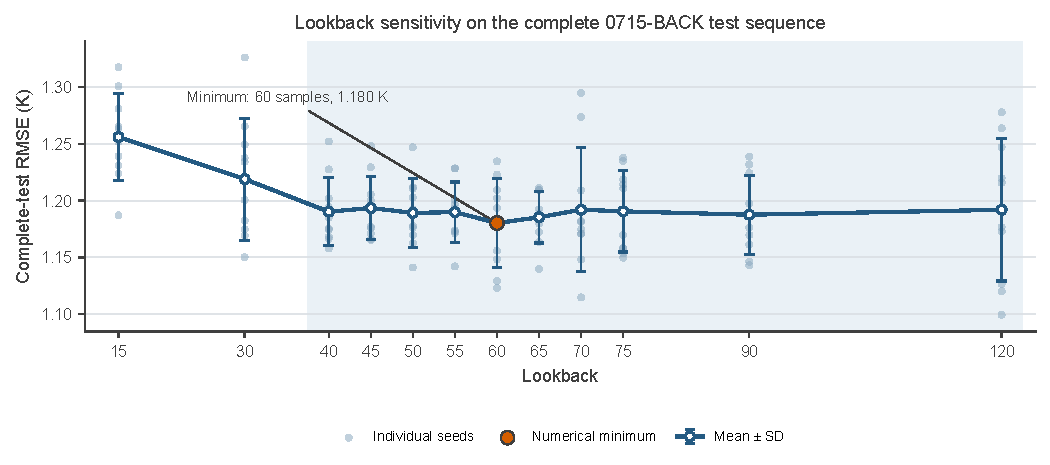
\includegraphics[width=0.97\textwidth]{figures/lookback_sensitivity_complete_test.pdf}
  \caption{未来15步$\Thv$预测的历史窗口敏感性。浅色点为各随机种子，折线和误差棒为均值$\pm$标准差。所有数值来自Original 0715-BACK完整测试序列，而非离散抽取的快速降温子集。}
  \label{fig:lookback}
\end{figure*}

\subsection{模型架构比较}

为隔离架构效应，本组实验统一使用20个原始历史变量、相同未来控制、隐藏维度和训练协议。图\ref{fig:architecture}与表\ref{tab:architecture}给出结果。并行GRU--MLP--GNN获得最低平均RMSE 1.142 K，并行GRU--单调KAN--GNN为1.150 K；两者分别较GRU基线降低2.92\%和2.25\%。对应95\%均值置信区间彼此重叠，因此现有证据不能声称MLP或KAN在精度上显著胜出。

并行结构的四种组合均处于1.142--1.152 K，而串行MLP--GNN--GRU和串行KAN--GNN--GRU分别升至2.381和2.154 K。串行结构对随机初始化也更敏感，其中MLP串行模型出现4.590 K的单种子结果。该现象说明，把每个历史时刻先压缩为图状态再送入GRU，会丢失对缓慢趋势有用的原始连续信息，并使边门控误差沿时间传播；并行结构保留历史直通路径，因此更稳健。

\begin{figure*}[t]
  \centering
  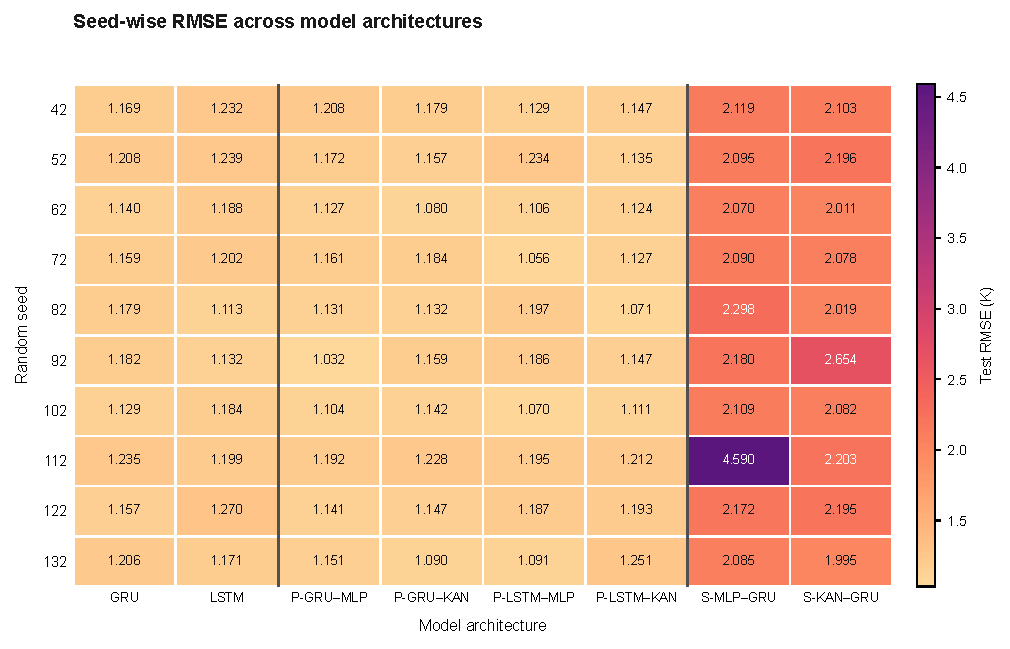
\includegraphics[width=0.96\textwidth]{figures/model_architecture_seed_rmse_heatmap.pdf}
  \caption{不同随机种子下各模型在Original 0715-BACK完整测试序列上的RMSE。列顺序依次为循环基线、并行结构和串行结构。}
  \label{fig:architecture}
\end{figure*}

\begin{table*}[t]
\centering
\caption{模型架构比较（完整测试集，10个随机种子）。}
\label{tab:architecture}
\begin{threeparttable}
\begin{tabular}{@{}lrrrrr@{}}
\toprule
模型 & 参数量 & RMSE (K) & MAE (K) & P95 (K) & $R^2$ \\
\midrule
GRU基线 & 26,657 & $1.176\pm0.033$ & $0.323\pm0.025$ & $1.304\pm0.233$ & 0.99786 \\
LSTM基线 & 32,161 & $1.193\pm0.048$ & $0.337\pm0.034$ & $1.450\pm0.129$ & 0.99780 \\
并行GRU--MLP--GNN & 87,059 & $\mathbf{1.142\pm0.049}$ & $0.302\pm0.014$ & $1.338\pm0.145$ & 0.99798 \\
并行GRU--单调KAN--GNN & 87,193 & $1.150\pm0.044$ & $\mathbf{0.294\pm0.012}$ & $\mathbf{1.248\pm0.172}$ & 0.99795 \\
并行LSTM--MLP--GNN & 92,563 & $1.145\pm0.062$ & $0.308\pm0.011$ & $1.322\pm0.137$ & 0.99797 \\
并行LSTM--单调KAN--GNN & 92,697 & $1.152\pm0.053$ & $0.302\pm0.017$ & $1.324\pm0.151$ & 0.99795 \\
串行MLP--GNN--GRU & 91,411 & $2.381\pm0.779$ & $0.936\pm0.509$ & $4.814\pm1.957$ & 0.99040 \\
串行单调KAN--GNN--GRU & 91,545 & $2.154\pm0.193$ & $0.765\pm0.128$ & $4.177\pm0.277$ & 0.99278 \\
\bottomrule
\end{tabular}
\begin{tablenotes}[flushleft]\footnotesize
\item 注：TCN仅作为探索性实验，不纳入主模型比较；P95为绝对误差的95百分位。
\end{tablenotes}
\end{threeparttable}
\end{table*}

\subsection{模型选择依据}

若只追求当前测试集最低RMSE，应选择并行GRU--MLP--GNN；若还要求阀门边函数满足局部导通单调性，则并行GRU--单调KAN--GNN提供更明确的结构解释，并取得更低的MAE和P95。两者RMSE仅相差0.008 K，小于跨种子标准差。基于这一精度--解释性折中，本文不宣称KAN精度更优，而将并行GRU--单调KAN--GNN作为后续物理特征和反事实实验的固定载体。最终投稿模型需在反事实外推实验完成后，再决定保留KAN还是回到MLP边门控。

\subsection{物理特征消融}

特征消融固定采用并行GRU--单调KAN--GNN，并通过通道掩码保持各配置可训练参数数目一致。完整20特征模型的RMSE为$0.960\pm0.033$ K，相比只使用20个原始变量的$1.181\pm0.050$ K降低18.75\%，10个配对种子全部改善，Holm校正后的Wilcoxon检验$p=0.0176$。删除目标历史动态组后，RMSE升至1.057 K，较完整模型恶化10.13\%，且校正后$p=0.0313$，是当前唯一具有稳定独立贡献的特征组。删除模组阀门动态和模组耦合后，RMSE分别恶化5.27\%和4.36\%，但多重比较校正后尚未达到0.05显著性水平。

其余低阶物理代理的独立删除没有显著恶化完整模型；删除混气热驱动组甚至得到0.946 K，但其置信区间跨越零差异。这表明这些变量可能与原始温压流高度冗余，不能因名称具有物理含义就默认保留。两项表观漏热特征使均值由0.960 K变为0.948 K，同样未形成稳定证据。当前更合理的下一步是围绕“目标历史动态+模组阀门动态+模组耦合”建立精简组合，而不是继续叠加特征。

\begin{table}[t]
\centering
\caption{关键特征配置的完整测试RMSE。}
\label{tab:featureablation}
\begin{tabular}{@{}p{4.35cm}r@{}}
\toprule
配置 & RMSE (K) \\
\midrule
仅20个原始变量 & $1.181\pm0.050$ \\
完整20个构造特征 & $0.960\pm0.033$ \\
删除目标历史动态 & $1.057\pm0.065$ \\
删除模组阀门动态 & $1.011\pm0.051$ \\
删除模组耦合 & $1.002\pm0.043$ \\
增加2个表观漏热特征 & $0.948\pm0.047$ \\
\bottomrule
\end{tabular}
\end{table}

\section{讨论}\label{sec:discussion}

\subsection{为什么60点历史窗口足够}

模组降温具有明显热惯性，过短窗口无法区分“温度相近但趋势不同”的状态；从15点增加到60点持续改善说明模型确实利用了历史，而不是完全复制当前$\Thv$。当窗口超过60点后，新增历史与当前状态的相关性降低，且GRU需要在更长序列中保留有效梯度，因此平均误差进入波动平台。60点不是可推广到其他设备的物理常数，而是当前采样周期、目标时距和数据覆盖下的经验最优值。

\subsection{为什么并行结构优于串行结构}

串行图--GRU假设每一时刻都可以先被压缩成一个足够的拓扑状态，再由GRU学习这些状态的演化。这一假设对当前数据过强：部分节点缺少独立流量或温度测量，图编码依赖共享上下文；重复压缩会丢失原始测点的细微趋势。并行结构把GNN定位为“拓扑校正项”，而不是历史信息的唯一入口，因此在固定图存在近似误差时仍能依赖GRU恢复趋势。这一解释与串行模型误差和种子方差同时增大的现象一致。

\subsection{精度、噪声与可用性边界}

测试集上的最佳完整特征模型RMSE约0.96 K，MAE约0.22 K。该水平明显优于1.978 K的持久性基线，但仍不能仅凭全局$R^2\approx0.999$判断已达到传感器噪声极限：完整温度曲线跨度大，$R^2$会被总体降温趋势放大；最大绝对误差仍约20 K，说明少数转折或异常阶段尚未解决。投稿前需要结合传感器标称精度、重复测量波动和局部窗口误差，才能论证噪声下限。

当前模型可在给定未来15步阀门序列时直接输出$t+15$的$\Thv$，但尚不能一次生成每个中间时刻的完整未来温度曲线。若用于未来控制序列评估，应增加多时距解码头，同时预测$t+1$至$t+H$并采用联合损失；在此之前，本文只把模型描述为“具备控制条件输入的开环预测代理”，不声称已经完成MPC部署。

\subsection{待完成的关键实验}

首先，需要以预先定义的阀门有效域构造反事实样本，分别增加3\%和5\%开度，报告温度响应方向违反率、违反幅值以及预测精度变化。该实验的主要目的应是评价分布外物理一致性，而不是强求同分布RMSE进一步下降。其次，应基于当前消融结果训练精简特征组合，并与完整20特征模型做10种子配对比较。再次，应补充代表性完整曲线、转折局部图和推理时延；若最终目标是输出完整未来曲线，还需增加多时距预测和误差随时距变化实验。最后，当前只有一个独立测试批次，后续应至少增加一个完全未参与开发的运行批次，以检验结论是否依赖0715-BACK的复温--再降温轨迹。

\section{结论}\label{sec:conclusion}

本文针对模组常规降温过程中的迟滞、分级阀门耦合和有限工况覆盖问题，构建了历史--拓扑并行多步温度预测框架。模型使用60点历史测量编码长期趋势，以固定有向GNN表达工艺连接，以未来15步阀门序列描述已知控制，并通过残差目标和快速降温加权Huber损失抑制平稳样本带来的零变化偏置。完整测试结果表明，60点历史窗口在当前搜索范围内获得最低平均RMSE；并行图--时序结构稳定优于循环基线和串行图--时序结构。MLP边门控取得最低RMSE，而单调KAN边门控在相近RMSE下取得更低MAE和P95，并提供局部阀门导通单调性。物理特征整体改善了跨批次测试误差，但可靠收益主要来自目标历史动态，其他代理量仍需精简组合与反事实实验验证。因而，本文当前最有力的结论是并行表征策略和因果实验协议的有效性，而不是某一复杂模块的绝对优势。

\section*{数据可用性声明}
原始运行数据涉及设备运行信息，暂不公开。在满足机构数据管理要求的前提下，可向通讯作者提出合理申请。用于复现实验的数据处理逻辑、模型配置和去标识化示例数据的公开范围将在投稿前确定。

\section*{利益冲突声明}
作者声明不存在可能影响本文工作的已知财务利益或个人关系。

\section*{作者贡献}
\todo{按Conceptualization、Methodology、Software、Data curation、Validation、Formal analysis、Visualization、Writing--original draft、Writing--review \& editing、Supervision和Funding acquisition填写。}

\section*{致谢}
\todo{补充项目、平台与人员支持。}

\bibliographystyle{cas-model2-names}
\bibliography{references}

\end{document}
